\documentclass[10pt,UTF8]{book} %% ctexart

\title{\textbf{操作系统}}
\author{钱锋\thanks{Email: strik0r.qf@gmail.com}${}^,$\thanks{
    西北工业大学软件学院, School of Software, Northwestern Polytechnical University, 西安 710072
}}

\usepackage{ctex}
\usepackage{graphicx}
\usepackage[toc]{multitoc}
\usepackage{amsthm, amssymb, amsmath, mathrsfs, mhchem}
\usepackage{tikz,circuitikz}
\usetikzlibrary{decorations.markings, angles, quotes, arrows.meta}
\usepackage{pgfplots}
\usepackage{subcaption}
\usepackage{tikz-3dplot}
\usepackage{extpfeil}
\usepackage{diagbox}
\usepackage{float}
\usepackage{hyperref}
\hypersetup{hidelinks,
    colorlinks = true,
    allcolors = black,
    pdfstartview = Fit,
    breaklinks = true}
\usepackage{caption}
\usepackage{enumitem}
\usepackage{siunitx}
% 定义带圆圈的数字命令
\newcommand{\circled}[1]{\textcircled{\small #1}}

\usepackage{fancyhdr} % 用于自定义页眉页脚


% 设置页眉页脚样式
\fancypagestyle{plain}{%
    \fancyhf{} % 清空页眉页脚
    \fancyhead[RO,LE]{·\thepage·} % 页眉显示页码, RO表示奇数页右侧, LE表示偶数页左侧
    \fancyhead[LO]{\nouppercase{\rightmark}} % 页眉显示小节标题, LO表示奇数页左侧
    \fancyhead[RE]{\nouppercase{\leftmark}} % 页眉显示章节标题, RE表示偶数页右侧
    \renewcommand{\headrulewidth}{0.4pt} % 设置页眉横线的宽度
    \renewcommand{\footrulewidth}{0pt} % 取消页脚横线
}

\renewcommand{\headrule}{\hrule width\textwidth height\headrulewidth\vskip-\headrulewidth}

% % 取消奇偶页的页眉偏移
% \fancyhfoffset[RO,LE]{0pt}

% % 取消奇偶页的页眉偏移
% \fancyhfoffset[RO,LE]{0pt}

% 定义取消页眉的命令
\newcommand{\cancelheader}{%
    \fancyhead{} % 清空页眉
    \renewcommand{\headrulewidth}{0pt} % 取消页眉横线
    \renewcommand{\footrulewidth}{0pt} % 设置页脚横线的宽度
}

\renewcommand{\chaptermark}[1]{\markboth{第 \thechapter 章 \hspace{1em} #1}{}}
\renewcommand{\sectionmark}[1]{\markright{\thesection \, #1}}
\usepackage{titlesec} % 定义标题样式

% 设置 chapter 标题样式
\titleformat{\chapter}[hang]{\centering\heiti\Large\bfseries}{第\,\thechapter\,章}{1em}{}

% 定义 section 标题格式
\titleformat{\section}[hang]{\heiti\centering\large\bfseries}{\thesection}{1em}{}

% 定义 subsection 标题格式
\titleformat{\subsection}[hang]{\heiti\bfseries}{\textbf{\thesubsection}}{1em}{}

% 定义 subsubsection 标题格式
\setcounter{secnumdepth}{3}
\renewcommand\thesubsubsection{\arabic{subsubsection}.}
\titleformat{\subsubsection}[hang]{\kaishu}{\quad\quad\thesubsubsection\,\,}{0em}{}

% % 重新定义 textbf
% \let\oldtextbf\textbf
% \renewcommand{\textbf}[1]{{\heiti\oldtextbf{#1}}}

% % 在导言区重新定义 \normalsize 命令
% \makeatletter
% \renewcommand\normalsize{%
%    \@setfontsize\normalsize{10.5pt}{12pt}%
%    \abovedisplayskip 8\p@ \@plus2\p@ \@minus5\p@
%    \abovedisplayshortskip \z@ \@plus3\p@
%    \belowdisplayshortskip 6\p@ \@plus3\p@ \@minus3\p@
%    \belowdisplayskip \abovedisplayskip
%    \let\@listi\@listI}
% \makeatother



% 设置页边距和对齐
% \usepackage[
%     paperwidth=185mm,
%     paperheight=260mm,
%     top=35mm,
%     bottom=25mm,
%     left=18mm,
%     right=18mm,
%     footskip=15mm % 通过这里的值来调整页脚与正文内容的垂直距离
% ]{geometry}

\usepackage[
    paperwidth=210mm,
    paperheight=297mm,
    top=40mm,
    bottom=31.8mm,
    left=25.4mm,
    right=25.4mm,
    footskip=15mm % 通过这里的值来调整页脚与正文内容的垂直距离
]{geometry}

% \usepackage[
%     paperwidth=195mm,
%     paperheight=270mm,
%     top=40mm,
%     bottom=25mm,
%     left=23.5mm,
%     right=23.5mm,
%     footskip=15mm % 通过这里的值来调整页脚与正文内容的垂直距离
% ]{geometry}
\usepackage{mdframed}
\mdfsetup{
  linewidth=0.4pt,
  frametitlebackgroundcolor=white, % 或者 transparent
  frametitlefont=\heiti\bfseries,
  frametitleaboveskip=10pt,
  frametitlebelowskip=5pt,
  frametitlealignment=\raggedright % 新增此行
}
\usepackage{fontspec}
% 设置 Menlo 字体
\setmonofont{Menlo}
\usepackage{fancyvrb}
\usepackage{xcolor}
\usepackage{listings}

\definecolor{string}{HTML}{067D17}
\definecolor{comment}{HTML}{8C8C8C}
\definecolor{keyword}{HTML}{0033B3}
\definecolor{class_field}{HTML}{871094}

\lstset{breaklines}
%这条命令可以让LaTeX自动将长的代码行换行排版
\lstset{extendedchars=false}
%这一条命令可以解决代码跨页时,章节标题,页眉等汉字不显示的问题
\lstset{escapeinside={(*}{*)}}

\lstset{
    basicstyle=\small\ttfamily\heiti,
    numbers=left,
    numberstyle=\scriptsize\fontspec{Menlo}, % 使用 Menlo 字体
    stepnumber=1,
    numbersep=8pt,
    frame=leftline,
    xleftmargin=2em, % 调整代码块的左边界
    framexleftmargin=0pt, % 调整边框的位置
    breaklines=true,
    keywordstyle=\bfseries\color{keyword},          % keyword style
    commentstyle=\heiti\color{comment},       % comment style
    stringstyle=\color[HTML]{067D17},
    showstringspaces=false,
    % string literal style
    % escapeinside={\%*}{*)},            % if you want to add LaTeX within your code
    % morekeywords={}               % if you want to add more keywords to the set
}

\usepackage{smartdiagram}
\usepackage{subcaption}
\usepackage{tasks}
\everymath{\displaystyle}

\begin{document}

\newtheoremstyle{mytheoremstyle}
    {1.5ex}                                         % Space above
    {1.5ex}                                         % Space below
    {}                                              % Font for body
    {}                                              % Indent amount
    {\bfseries}                                     % Font for head
    {}                                              % Punctuation after head
    {0.5em plus 0.2em minus 0.1em}                  % Space after head
    {\thmname{#1}\thmnumber{ #2}.\thmnote{ (#3).}}

\theoremstyle{mytheoremstyle}
\newtheorem{definition}{定义}[section]
\newtheorem{example}{例}[section]
\newtheorem{exercise}{习题}[section]
\newtheorem{code}{程序清单}[section]
\newtheorem*{result}{运行结果}

\newtheoremstyle{my2theoremstyle}
    {1.5ex}                                         % Space above
    {1.5ex}                                         % Space below
    {\kaishu}                                              % Font for body
    {}                                              % Indent amount
    {\bfseries}                                     % Font for head
    {}                                              % Punctuation after head
    {0.5em plus 0.2em minus 0.1em}                  % Space after head
    {\thmname{#1}\thmnumber{ #2}.\thmnote{ (#3).}}

\theoremstyle{my2theoremstyle}
\newtheorem{thm}{定理}[section]
\newtheorem{law}{定律}[section]
\newtheorem{educt}{推论}
\newtheorem{prop}{命题}
\newtheorem{lemma}{引理}
\newtheorem{axiom}{公理}
\newtheorem{property}{性质}

\newtheoremstyle{my4theoremstyle}
    {1.5ex}                                         % Space above
    {1.5ex}                                         % Space below
    {}                                              % Font for body
    {}                                              % Indent amount
    {\bfseries}                                     % Font for head
    {}                                              % Punctuation after head
    {0.5em plus 0.2em minus 0.1em}                  % Space after head
    {\thmname{#1}.}

\theoremstyle{my4theoremstyle} \newtheorem*{sol}{解}

\newtheoremstyle{my3theoremstyle}
    {1.5ex}                                         % Space above
    {1.5ex}                                         % Space below
    {}                                              % Font for body
    {}                                              % Indent amount
    {\kaishu}                                       % Font for head
    {}                                              % Punctuation after head
    {0.5em plus 0.2em minus 0.1em}                  % Space after head
    {\thmname{#1}\thmnumber{ #2}.\thmnote{ (#3).}}

\theoremstyle{my3theoremstyle} \newtheorem*{remark}{注}
\newtheorem*{cmt}{评注}
\pagestyle{empty}
\begin{titlepage}
    \thispagestyle{empty}
    \centering
        \vspace*{2cm}
        
\includegraphics[width=0.5\textwidth]{pic/npu_2.png}\par
        \vspace{1em}
        
\includegraphics[width=0.5\textwidth]{pic/npu_1.png}\par
    \vspace{1em}
        \begin{center}
            \Huge \heiti \textbf{操作系统}

            Operating System
        \end{center}
        \vspace{17em}
        \begin{center}
        \songti
        \kaishu 软件学院 \, \heiti\textbf{钱锋} \quad \songti 编
        \vspace{0.5em}

    \today
    \end{center}
\end{titlepage}
\cleardoublepage
\maketitle
\cleardoublepage

\frontmatter
\newpage
\pagestyle{plain}
\makeatother

% 设置目录页的页码格式
\addtocontents{toc}{\protect\thispagestyle{empty}}
\pagestyle{plain}
{\tableofcontents}
\newpage
\thispagestyle{empty}
\cleardoublepage % 确保正文从奇数页开始


% 设置章节标题页的页眉和页脚为空白页样式
\makeatletter
\let\ps@plain\ps@empty
\makeatother

\mainmatter
\chapter{操作系统引论}

\textbf{操作系统} (operating system, OS) 是配置在计算机硬件上的第一层软件,
是计算机软硬件资源的管理者.
它为用户提供一台等价的扩展机器 (extended machine) 或虚拟机 (virtual machine),
是最重要、最基本、最复杂的系统程序, 控制应用程序执行的程序.

\section{操作系统的目标与作用}

\subsection{操作系统的目标}

在计算机上配置操作系统, 其主要目标是实现方便性、有效性、可扩充性、开放性.

\subsection{操作系统的作用}

可以从人机交互、资源管理及资源抽象等不同方面来分析 OS 在计算机系统中所占的作用.
\begin{enumerate}[itemsep=0pt]
    \item 人机交互: \textbf{操作系统作为用户与计算机硬件系统之间的接口}.
    OS 处于用户与计算机硬件系统之间, 用户通过使用 OS 来使用计算机硬件系统.
    \item 资源管理: \textbf{操作系统作为计算机系统资源的管理者}.
    计算机系统的各种硬件资源和软件资源归纳起来可以分为处理机、存储器、I/O 设备以及
    信息 (数据和程序) 四类, OS 的主要功能正是对这四类资源进行有效的管理.
    \begin{itemize}[itemsep=0pt]
        \item 处理机管理负责处理机的分配与控制;
        \item 存储器管理负责内存的分配与回收;
        \item I/O 设备管理负责 I/O 设备的分配 (回收) 与操纵;
        \item 文件管理负责文件的读取、共享与保护等;
        \item 对共享资源的使用请求进行授权, 以协调多用户对共享资源的使用;
    \end{itemize}
    \item 资源抽象: \textbf{操作系统实现了对计算机资源的抽象}.
    OS 是铺设在计算机硬件上的多层软件的集合, 它增强了系统的功能, 也隐藏了对硬件
    操作的具体细节, 实现了对计算机硬件操作的多个层次的抽象模型.
\end{enumerate}

\begin{figure}[H]
    \centering

\tikzset{every picture/.style={line width=0.75pt}} %set default line width to 0.75pt        

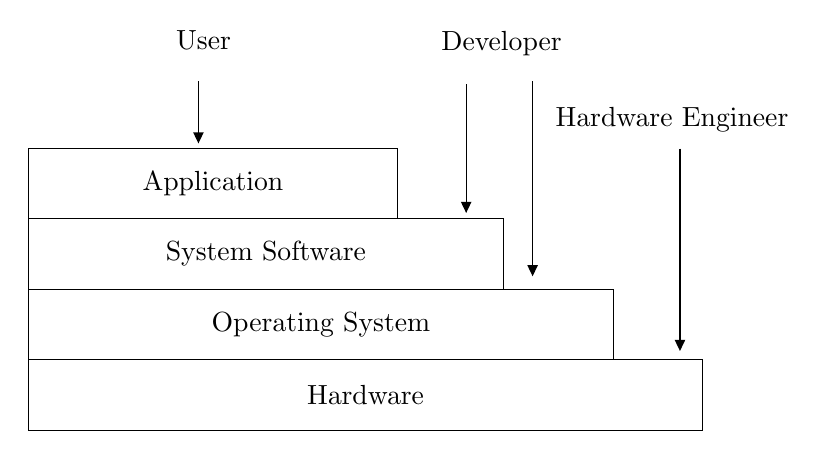
\begin{tikzpicture}[x=0.75pt,y=0.75pt,yscale=-1,xscale=1]
%uncomment if require: \path (0,300); %set diagram left start at 0, and has height of 300

%Straight Lines [id:da6901240446201179] 
\draw    (350,94.5) -- (350,121.5) ;
\draw [shift={(350,124.5)}, rotate = 270] [fill={rgb, 255:red, 0; green, 0; blue, 0 }  ][line width=0.08]  [draw opacity=0] (5.36,-2.57) -- (0,0) -- (5.36,2.57) -- cycle    ;
%Straight Lines [id:da9982243945284205] 
\draw    (479,96) -- (479,155) ;
\draw [shift={(479,158)}, rotate = 270] [fill={rgb, 255:red, 0; green, 0; blue, 0 }  ][line width=0.08]  [draw opacity=0] (5.36,-2.57) -- (0,0) -- (5.36,2.57) -- cycle    ;
%Straight Lines [id:da8836809318744954] 
\draw    (511,94.5) -- (511,185.5) ;
\draw [shift={(511,188.5)}, rotate = 270] [fill={rgb, 255:red, 0; green, 0; blue, 0 }  ][line width=0.08]  [draw opacity=0] (5.36,-2.57) -- (0,0) -- (5.36,2.57) -- cycle    ;
%Straight Lines [id:da6563399166074272] 
\draw    (582,127) -- (582,221.5) ;
\draw [shift={(582,224.5)}, rotate = 270] [fill={rgb, 255:red, 0; green, 0; blue, 0 }  ][line width=0.08]  [draw opacity=0] (5.36,-2.57) -- (0,0) -- (5.36,2.57) -- cycle    ;

% Text Node
\draw    (268,228.75) -- (593,228.75) -- (593,262.75) -- (268,262.75) -- cycle  ;
\draw (430.5,245.75) node   [align=left] {\begin{minipage}[lt]{218.28pt}\setlength\topsep{0pt}
\begin{center}
Hardware
\end{center}

\end{minipage}};
% Text Node
\draw    (268,194.75) -- (550,194.75) -- (550,228.75) -- (268,228.75) -- cycle  ;
\draw (409,211.75) node   [align=left] {\begin{minipage}[lt]{189.04pt}\setlength\topsep{0pt}
\begin{center}
Operating System
\end{center}

\end{minipage}};
% Text Node
\draw    (268,160.75) -- (497,160.75) -- (497,194.75) -- (268,194.75) -- cycle  ;
\draw (382.5,177.75) node   [align=left] {\begin{minipage}[lt]{153pt}\setlength\topsep{0pt}
\begin{center}
System Software
\end{center}

\end{minipage}};
% Text Node
\draw    (268,126.75) -- (446,126.75) -- (446,160.75) -- (268,160.75) -- cycle  ;
\draw (357,143.75) node   [align=left] {\begin{minipage}[lt]{118.32pt}\setlength\topsep{0pt}
\begin{center}
Application
\end{center}

\end{minipage}};
% Text Node
\draw (335,69) node [anchor=north west][inner sep=0.75pt]   [align=left] {\begin{minipage}[lt]{24.26pt}\setlength\topsep{0pt}
\begin{center}
User
\end{center}

\end{minipage}};
% Text Node
\draw (462,69) node [anchor=north west][inner sep=0.75pt]   [align=left] {\begin{minipage}[lt]{49.22pt}\setlength\topsep{0pt}
\begin{center}
Developer
\end{center}

\end{minipage}};
% Text Node
\draw (516.5,106) node [anchor=north west][inner sep=0.75pt]   [align=left] {\begin{minipage}[lt]{90.61pt}\setlength\topsep{0pt}
\begin{center}
Hardware Engineer
\end{center}

\end{minipage}};


\end{tikzpicture}
\caption{操作系统作为用户与计算机硬件系统之间的接口}
\end{figure}

\section{操作系统的基本特性}

\subsection{并发}

并行是指两个或多个时间在同一时刻发生, \textbf{并发} (concurrence) 是指在一段时间内
宏观上有多个程序在同时运行.

\subsection{共享}
\subsection{虚拟}
\subsection{异步}

\begin{example}
    说明库函数与系统调用的区别与联系.
    \begin{cmt}
        \begin{enumerate}[label={$\left.\arabic*\right)$}, itemsep=0pt]
            \item {\color{red} \textbf{从属和运行环境不同}: 库函数是程序设计语言或应用程序的一部分, 
            可以运行在用户空间中,
            而系统调用则操作系统的一部分, 是内核为应用程序提供的接口, 运行在内核空间中.}
            \item \textbf{都可以被应用程序调用}: App 可以调用库函数, 也可以通过系统调用请求 OS 的服务.
            \item \textbf{系统调用比库函数更底层、更基本}: 库函数的执行如果需要 OS 的服务, 也需要通过系统调用来实现.
            {\color{red} 通常未使用系统调用的库函数执行效率比使用系统调用的高, 这是因为使用系统调用
            会涉及 CPU 在用户态与核心态之间的转换.}
        \end{enumerate}
    \end{cmt}
\end{example}

\chapter{进程的描述与控制}

\section{进程的描述}

\subsection{进程的定义与特征}

\textbf{进程} (process) 是程序的执行过程, 是系统进行资源分配和调度的一个独立单位.

为了使参与并发执行的每个程序 (含数据) 都能独立地运行, 在 OS 中必须为之配置一个
专门的数据结构, 称之为\textbf{进程控制块} (process control block, PCB).
OS 利用 PCB 来描述进程的基本情况和活动过程, 进而控制和管理进程.
所谓创建进程, 实际上是创建进程的 PCB, 所谓撤销进程, 实际上是撤销进程的 PCB.

进程的特征: 动态性 (程序是有序指令的集合, 是静态的, 进程是程序的一次执行过程,
是动态的)、并发性、独立性 (独立获得资源、独立接收调度)、异步性.

\subsection{进程的状态及其转换}

\begin{figure}[H]
    \centering
    \begin{center}
        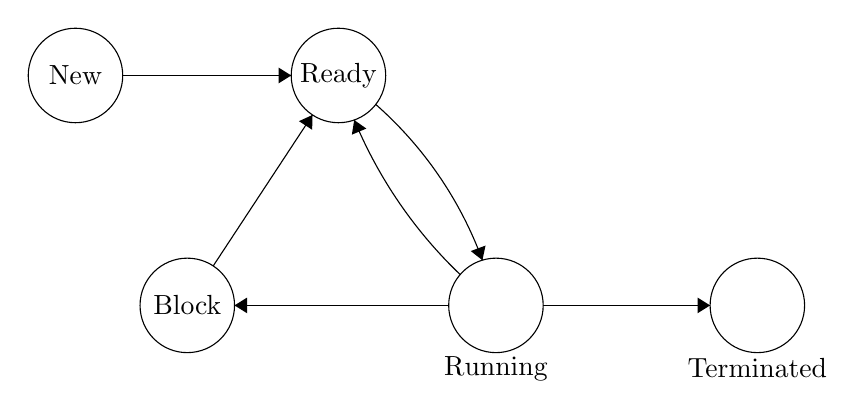
\begin{tikzpicture}[scale=0.2]
        \tikzstyle{every node}+=[inner sep=0pt]
        \draw [black] (36.9,-20.2) circle (3);
        \draw (36.9,-20.2) node {Ready};
        \draw [black] (27.3,-34.8) circle (3);
        \draw (27.3,-34.8) node {Block};
        \draw [black] (46.9,-34.8) circle (3);
        \draw (46.9,-38.8) node {Running};
        \draw [black] (20.2,-20.2) circle (3);
        \draw (20.2,-20.2) node {New};
        \draw [black] (63.5,-34.8) circle (3);
        \draw (63.5,-38.8) node {Terminated};
        \draw [black] (28.95,-32.29) -- (35.25,-22.71);
        \fill [black] (35.25,-22.71) -- (34.39,-23.1) -- (35.23,-23.65);
        \draw [black] (39.268,-22.038) arc (48.65002:20.16692:24.361);
        \fill [black] (46.04,-31.93) -- (46.24,-31) -- (45.3,-31.35);
        \draw [black] (43.9,-34.8) -- (30.3,-34.8);
        \fill [black] (30.3,-34.8) -- (31.1,-35.3) -- (31.1,-34.3);
        \draw [black] (23.2,-20.2) -- (33.9,-20.2);
        \fill [black] (33.9,-20.2) -- (33.1,-19.7) -- (33.1,-20.7);
        \draw [black] (44.629,-32.842) arc (-133.72846:-157.4546:28.941);
        \fill [black] (37.9,-23.03) -- (37.75,-23.96) -- (38.67,-23.57);
        \draw [black] (49.9,-34.8) -- (60.5,-34.8);
        \fill [black] (60.5,-34.8) -- (59.7,-34.3) -- (59.7,-35.3);
        \end{tikzpicture}
        \end{center}
    \caption{进程的状态及其转换}
    \label{进程的状态及其转换}
\end{figure}

\begin{itemize}[itemsep=0pt]
    \item \textbf{创建状态} (New): 系统创建进程 PCB, 并为其分配资源.
    \item \textbf{就绪状态} (Ready): 进程已经分配到除 CPU 以外的所有必要资源.
    \item \textbf{执行状态} (Running): 进程获得 CPU 后程序正在执行的状态.
    \item \textbf{阻塞状态} (Block): 正在执行的进程由于某事件的发生或者需要请求某系统资源
    而暂时无法运行的的状态.
    \item \textbf{终止状态} (Terminated): 进程运行结束, 或在运行过程中遇到不可修复的错误, 
    则系统回收资源.
\end{itemize}

\section{进程控制}

进程控制是进程管理中最基本的功能, 其负责创建新进程、终止已完成的进程、
将因发生异常情况而无法继续运行的进程置于阻塞状态、转换运行中进程的状态等,
总的来说, 进程控制的主要功能就是实现进程状态的转换.

进程控制一般是由 OS 内核中的原语来实现的. 原语的执行具有原子性,
即不允许中断, 只能一气呵成. 如果进程控制不通过允许实现, 而是允许中断的话,
则可能会导致 OS 中某些关键数据结构中的信息不统一的问题, 进而影响 OS 的工作.

\subsection{进程的创建}

\appendix
% 设置 chapter 标题样式
\titleformat{\chapter}[hang]{\centering\heiti\Large\bfseries}{附录\,\thechapter}{1em}{}
\renewcommand{\chaptermark}[1]{\markboth{附录 \thechapter\, #1}{}}

\onecolumn
\begin{thebibliography}{1}
    \addcontentsline{toc}{chapter}{参考文献}
    \bibitem{汤小丹}
    汤小丹等. 计算机操作系统: 慕课版 [M]. 北京: 人民邮电出版社, 2021.
    \bibitem{王道操作系统}
    王道论坛组. 2024 年操作系统考研复习指导 [M]. 北京: 电子工业出版社, 2022.
\end{thebibliography}

\newpage
\thispagestyle{empty}
\vspace*{5cm}
\begin{center}
    \includegraphics*[width=\textwidth]{pic/i_love_npu.jpeg}
    \large
    公诚勇毅 \quad 永矢毋忘

    中华灿烂 \quad 工大无疆
\end{center}
\vspace*{13em}
\begin{center}
    \small
    本文档由\textbf{钱锋}编写, 钱锋保留一切权利.

    文档中出现的部分素材来源于网络, 笔者承诺这些素材仅供学习交流之用, 
    它们的原作者保留一切权利.

    2023 年 \quad 西北工业大学 \quad 中国西安 
\end{center}

\end{document}